\documentclass{beamer}

\usepackage[spanish]{babel}
\usepackage[utf8]{inputenc}
\usepackage[T1]{fontenc}
\usepackage{amsmath,amssymb,amsfonts}
\usepackage{xcolor}
\usepackage{ragged2e}
\usepackage{etoolbox}
\usepackage{lipsum}
\usepackage[center]{caption}
\usepackage{biblatex}

\addbibresource{biblio.bib}

\usetheme{Madrid}
\title[Movimiento browniano]{Modelo a gran escala del movimiento Browniano \cite{Mazo_2014}, \cite{Schilling_Partzsch_Böttcher_2021}}
\author[Iván y Luis]{Iván Martinez Riveiro y Luis Lucas García}
\institute[UA]{Universidad de Alicante}
\date{14 de mayo de 2024}

\apptocmd{\frame}{}{\justifying}{}
\addtobeamertemplate{block begin}{}{\justifying} % Justify all blocks

\begin{document}
\begin{frame}
\maketitle
\end{frame}

\begin{frame}{Índice}
\tableofcontents
\end{frame}

\begin{frame}{El movimiento browniano}
\section{Introducción}

Si colocamos una partícula de pequeño tamaño y la observamos bajo el microscopio veremos pequeñas vibraciones. Estas se deben a la colisión con las moléculas que forman el medio y que vibran por el efecto de la temperatura.

\begin{block}{El movimiento browniano}
El movimiento browniano es el movimiento aparente aleatorio de una partícula en un medio (líquido o gas) debido a las colisiones con las partículas del medio.
\end{block}

\begin{figure}[h!]
\begin{center}
\includegraphics[scale=0.12]{2drandom.png}
\caption{Algunas trayectorias de movimiento browniano.}
\end{center}
\end{figure}
\end{frame}

\begin{frame}{La teoría}
A grandes rasgos, el movimiento browniano es como un camino aleatorio, pero en 2 dimensiones. Como tenemos muchas colisiones, se aproxima a una normal.

\begin{block}{La teoría de Einstein \cite{Einstein}}
Einstein encontró una expresión para el movimiento browniano. En 2 dimensiones esta se escribe como:

\begin{equation}
\rho (x, y, t) = \frac{N}{4 \pi D t}e^{- \frac{x^2 + y^2}{4Dt}} \, dxdy
\label{eq:randomWalk}
\end{equation}
\end{block}

\begin{figure}[h!]
\begin{center}
\includegraphics[scale=0.1]{distribuciones.png}
\caption{Algunas distribuciones de densidad para distintos parámetros.}
\end{center}
\end{figure}
\end{frame}

\begin{frame}{Distribución en polares}
Para nuestro experimento tendremos simetría circular, por lo que será conveniente transformar la distribución a coordenadas polares.

\begin{block}{Distribución polar}
Haciendo el cambio a polares e integrando sobre los ángulos se obtiene la siguiente distribución para el módulo de la distancia:

\begin{equation}
\rho (r, t) = \frac{N}{2Dt} r e^{- \frac{r^2}{4Dt}} \, dr
\label{eq:distribuciónR}
\end{equation}
\end{block}

El máximo de la distribución nos permite conocer D.

\begin{block}{Máximo de la distribución}
Derivando en función del radio obtenemos que se da un máximo en:

\begin{equation}
r_0 = \sqrt{2Dt}
\label{eq:difusionMax}
\end{equation}
\end{block}
\end{frame}

\begin{frame}{El coeficiente de difusión}
Gracias al movimiento browniano se han dado métodos de conocer el coeficiente de difusión.

\begin{block}{Cálculo de D}
Si suponemos un rozamiento de la forma de Stokes obtenemos dos formas de calcular el coeficiente de difusión.

\begin{equation}
D = \frac{\langle x^2 \rangle}{2t} \iff D = \frac{RT}{6 \pi \eta r N}
\label{eq:difusionT}
\end{equation}
\end{block}
\end{frame}

\begin{frame}{Objetivo}
\section{Desarrollo experimental}
Vamos a construir un modelo mecánico a gran escala del movimiento browniano. Esto nos permitirá estudiar los resultados teóricos.

\begin{block}{Objetivos}
Nuestros objetivos serán dos:

\begin{enumerate}
\item Comprobar que se cumple la distribución en \ref{eq:distribuciónR}.
\item Encontrar un coeficiente de difusión equivalente para nuestro sistema mecánico.
\end{enumerate}
\end{block}

\begin{figure}[h!]
\begin{center}
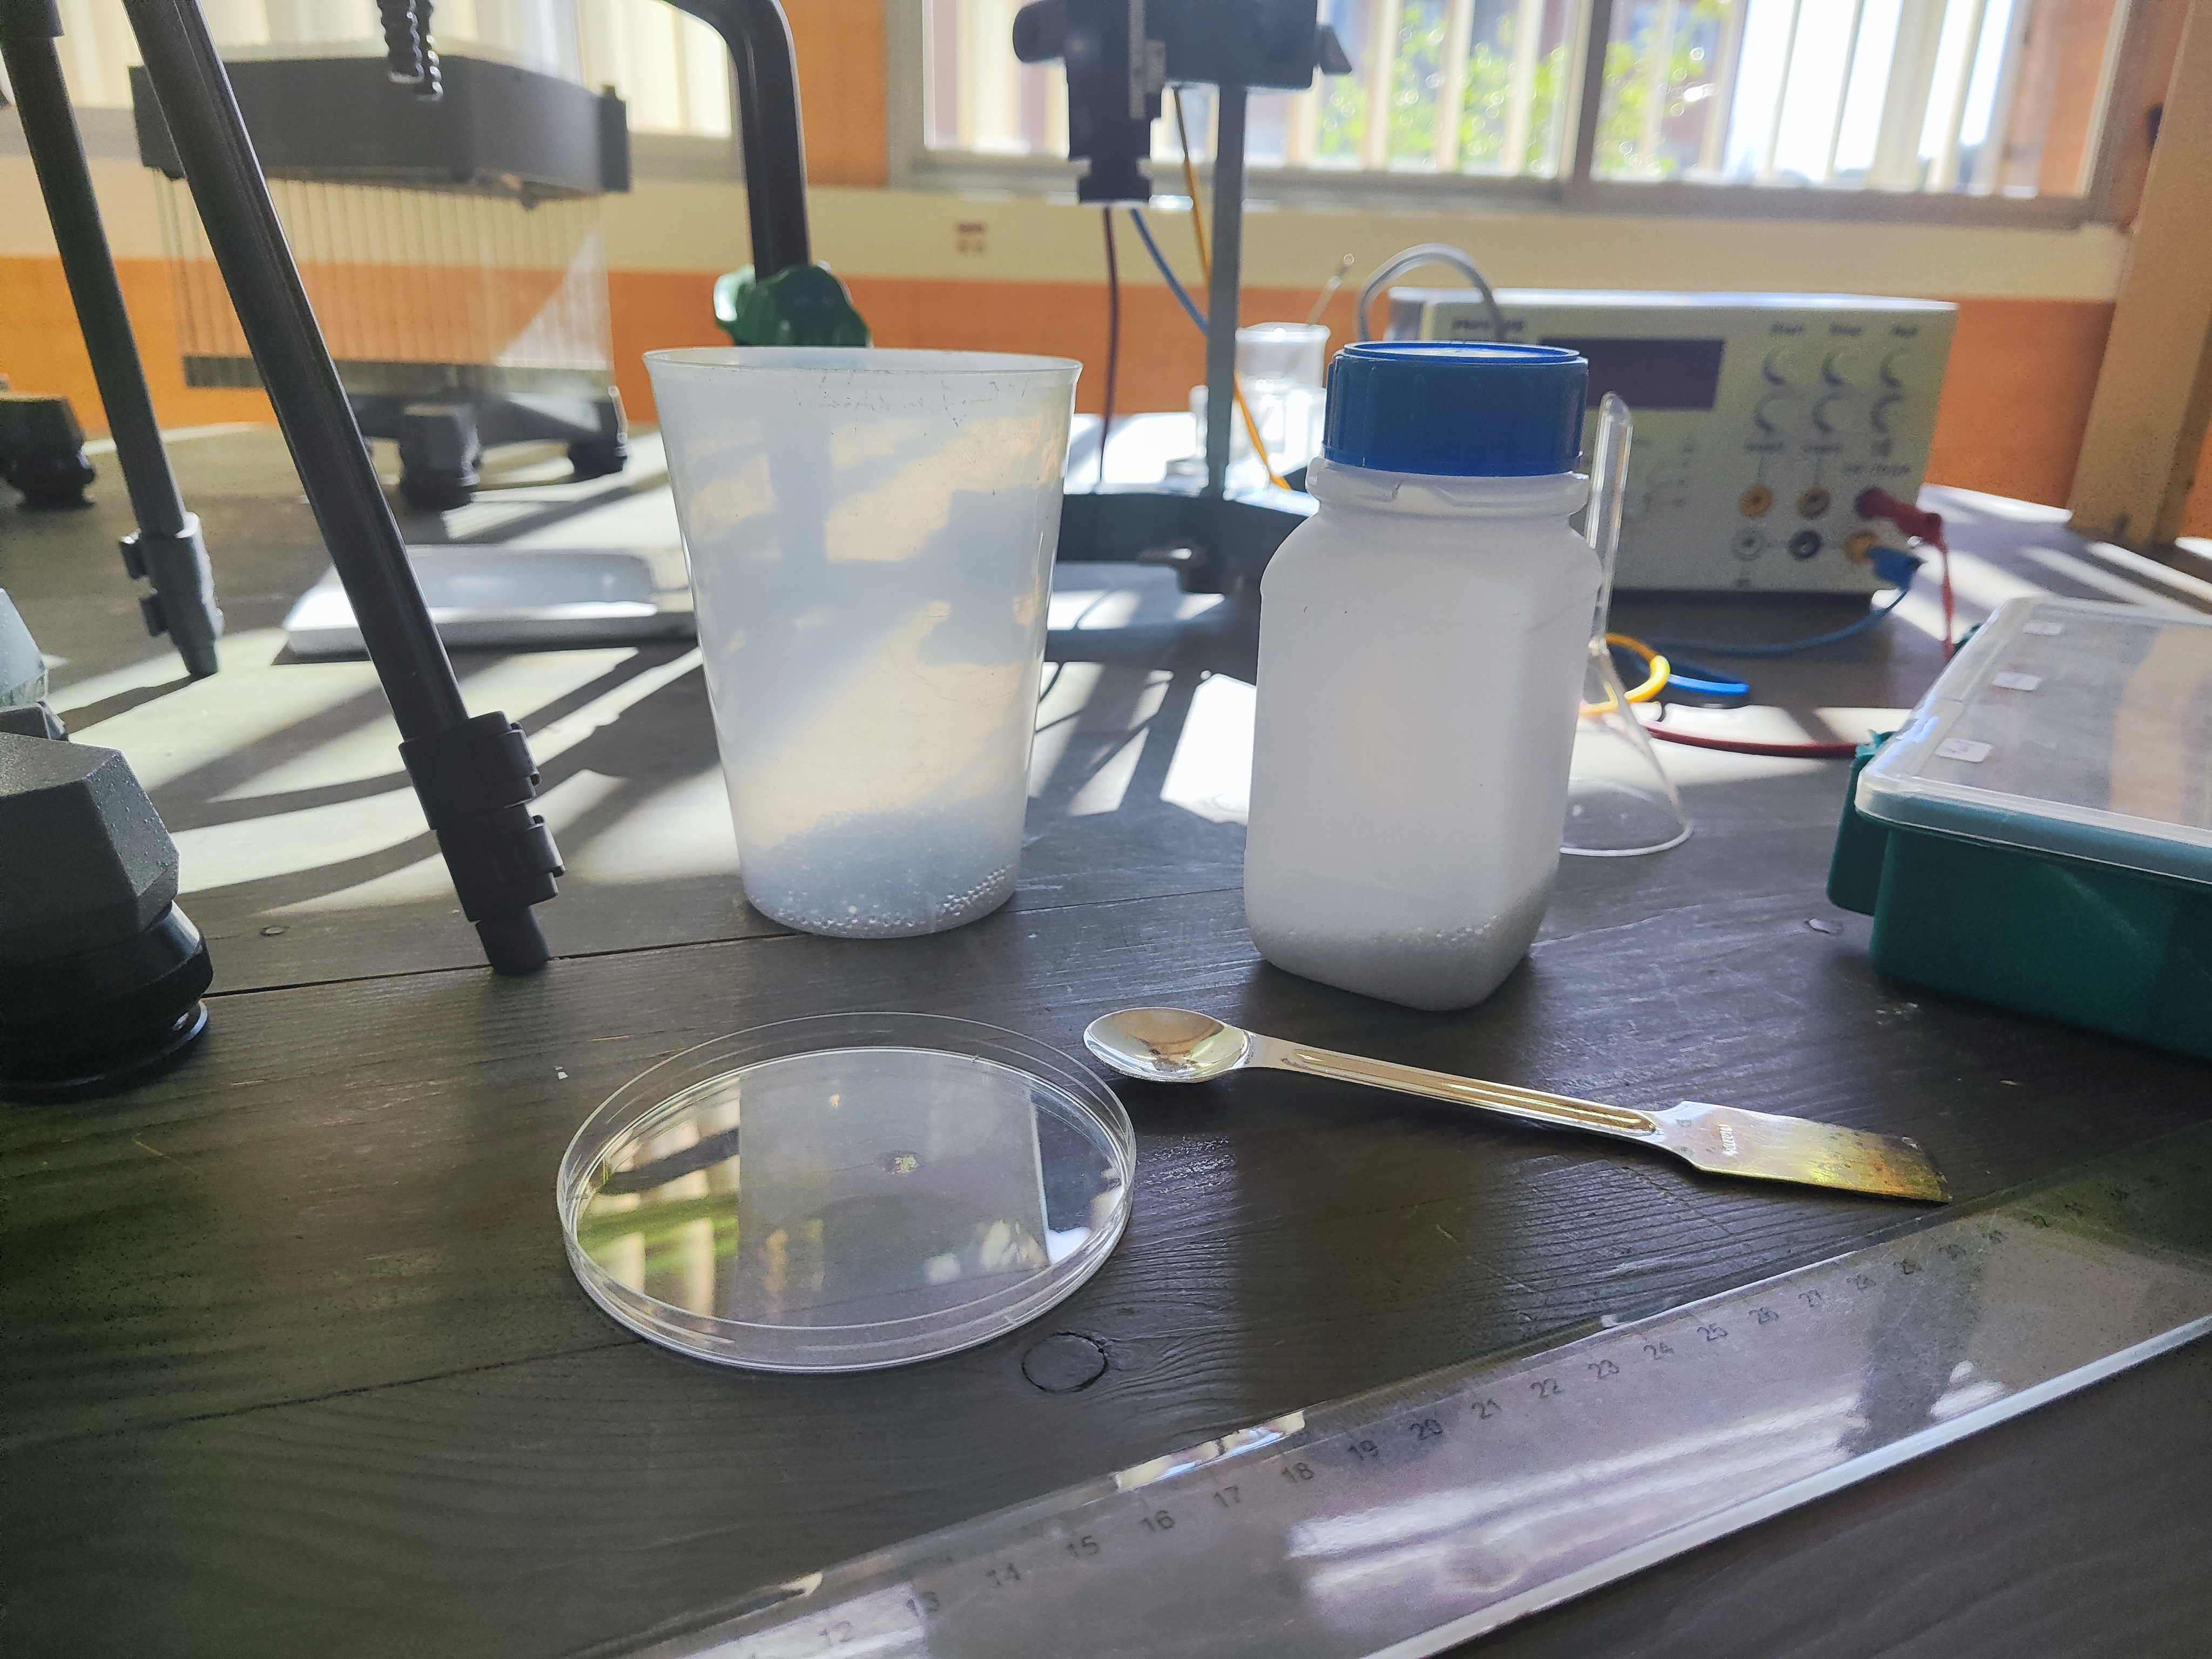
\includegraphics[scale=0.022]{materialLab.jpg}
\>
\includegraphics[scale=0.025]{bolitas.jpg}
\caption{Algunos de los instrumentos utilizados en el laboratorio.}
\end{center}
\end{figure}
\end{frame}

\begin{frame}{Montaje}
Contamos con un recipiente y su tapa, en el que pondremos unas bolitas pequeñas (las del experimento de Maxwell - Boltzmann) y otras más grandes y distinguibles, de metal.

Contamos con el agitador del experimento de Fermi - Dirac que hemos adaptado para que pueda mover nuestro recipiente. Tenemos también un trípode en el que colocar el móvil para grabar el movimiento.

\begin{figure}[h!]
\begin{center}
\includegraphics[scale=0.045]{modeloLab.jpg}
\>
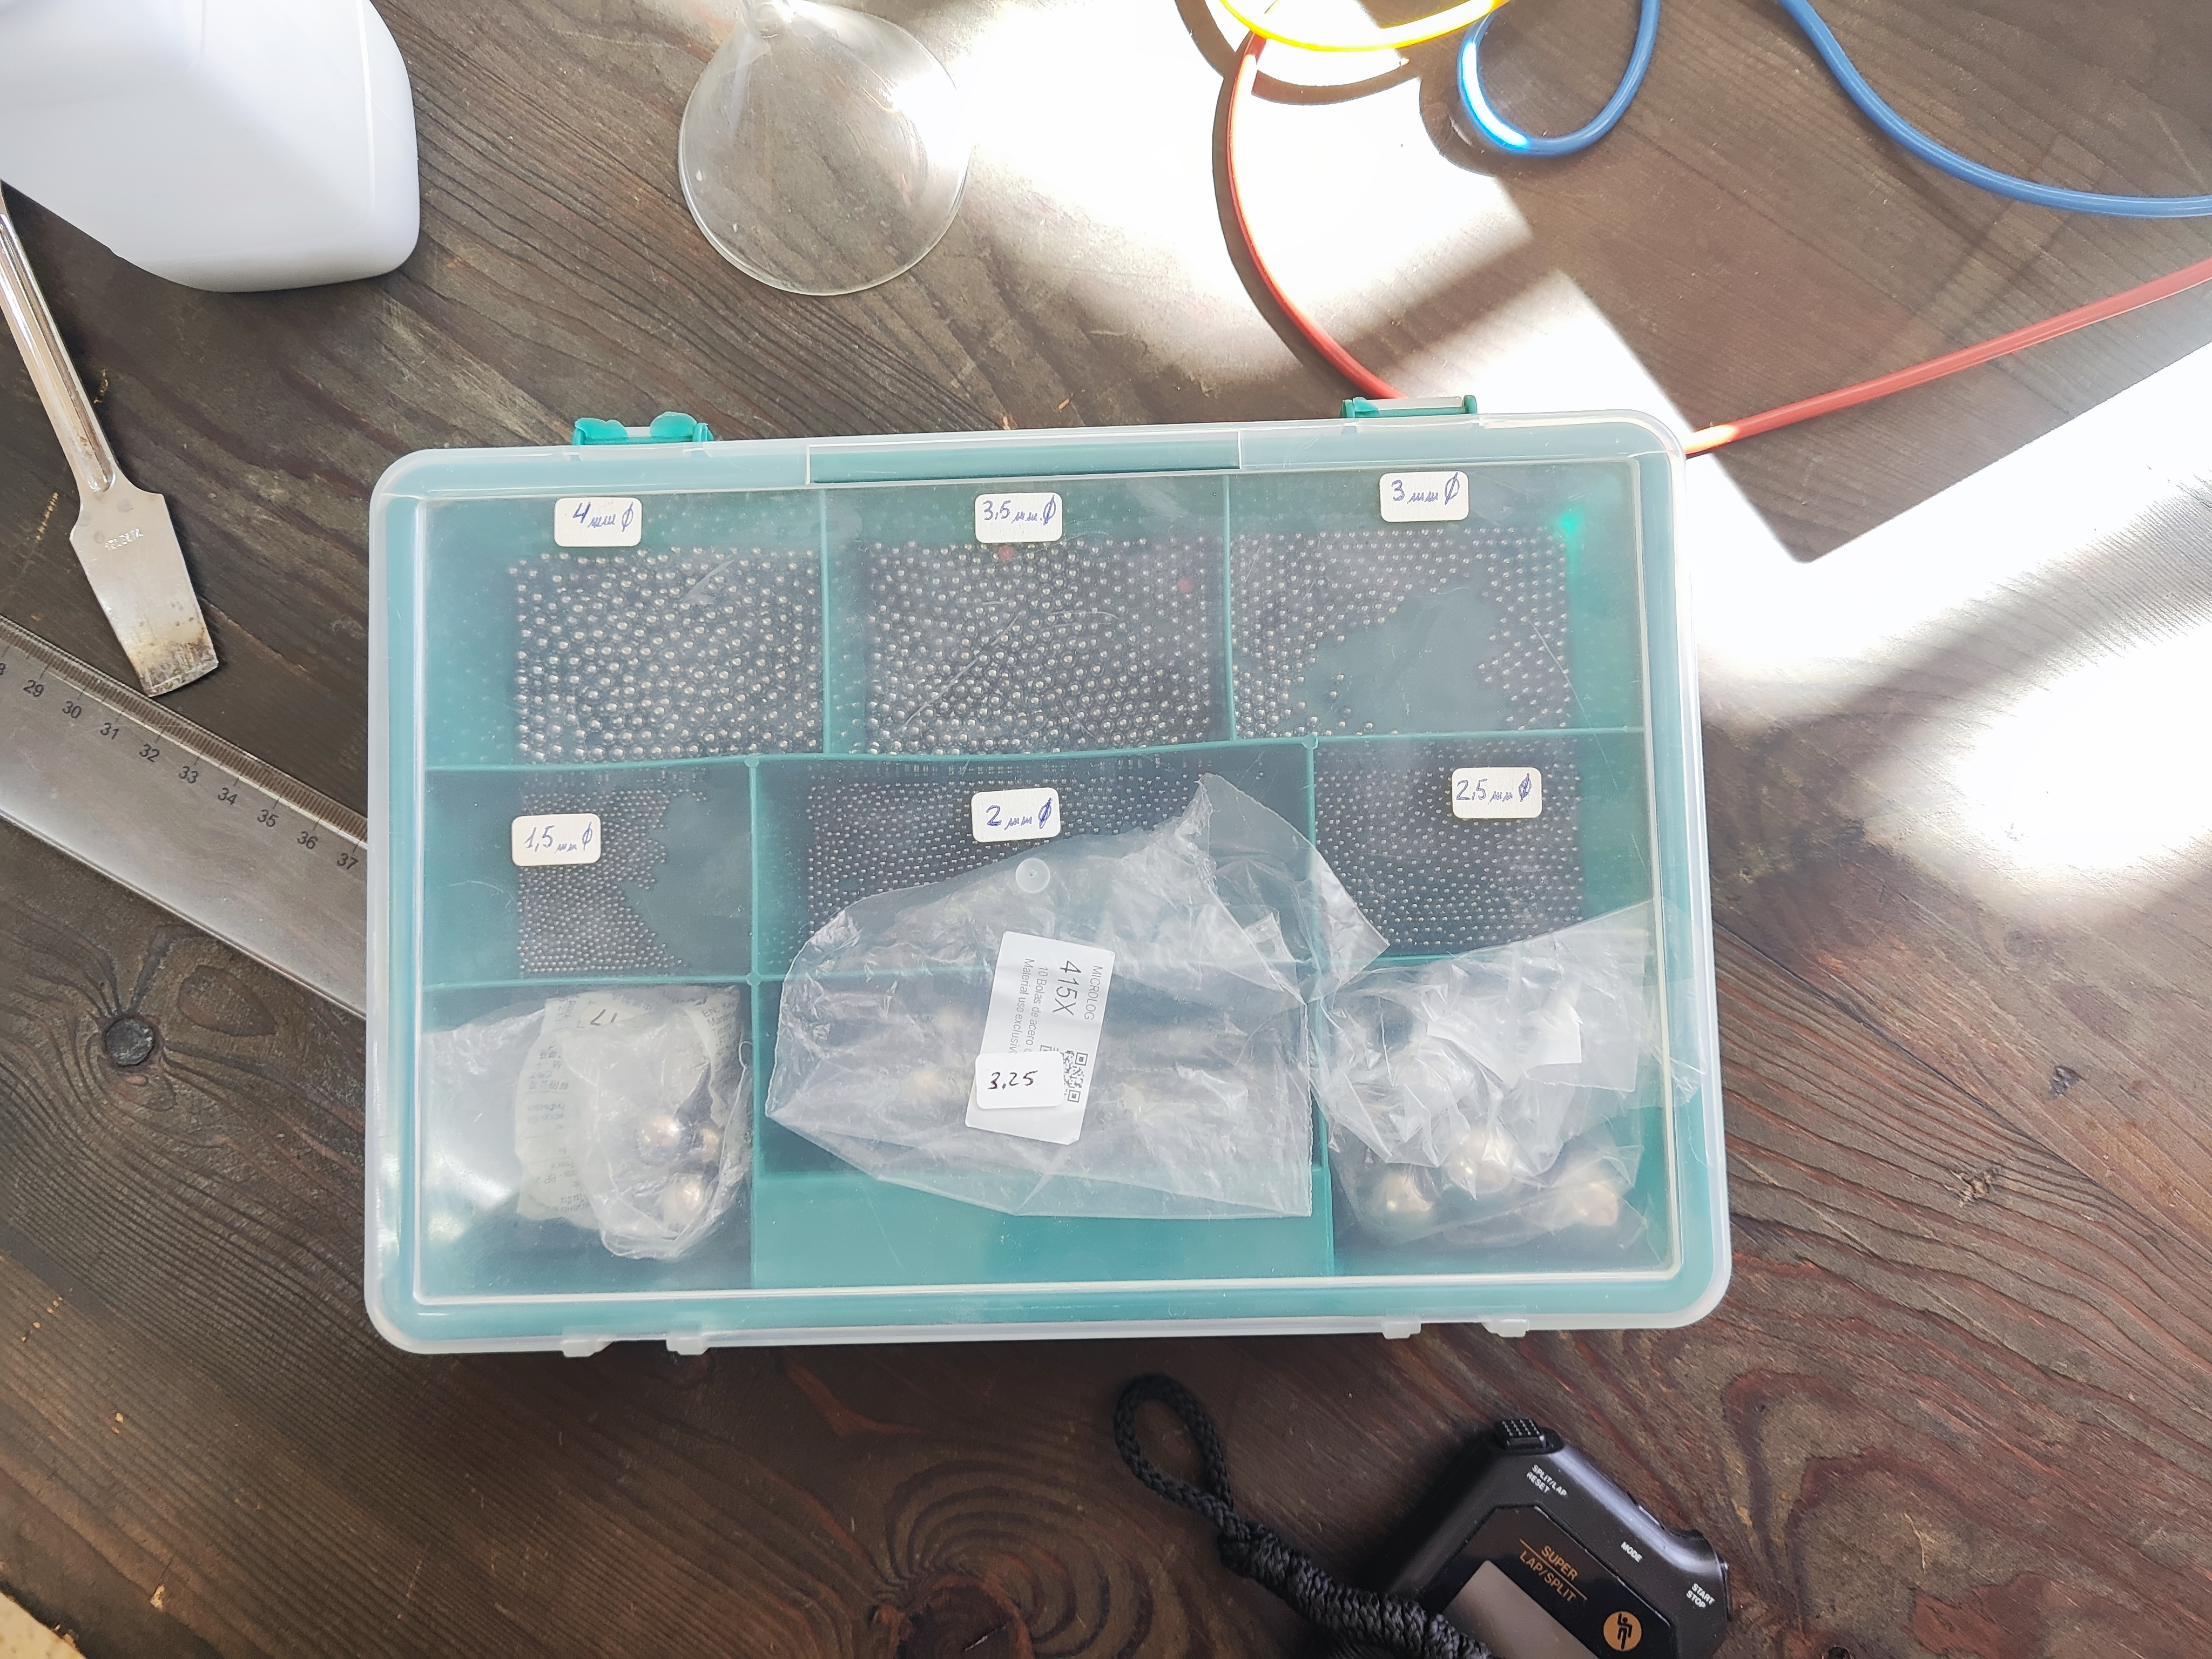
\includegraphics[scale=0.035]{modeloLab2.jpg}
\caption{Foto del dispositivo del experimento.}
\end{center}
\end{figure}
\end{frame}

\begin{frame}{Distribución experimental}
En esta parte vamos a ver qué resultados obtenemos de las medidas de distancia al centro para bolitas de metal en dos velocidades de vibración distintas. Para ello colocamos las varias bolitas en el centro y dejamos que el sistema evolucione unos cinco segundos, obteniendo:

\begin{figure}[h!]
\begin{center}
\includegraphics[scale=0.3]{Histograma resultados.png}
\caption{Histograma de los resultados. En naranja la correspondiente a la vibración más rápida.}
\end{center}
\end{figure}
\end{frame}

\begin{frame}{Comparación teórica}
Por la ecuación \ref{eq:difusionMax} podríamos ajustar la distribución \ref{eq:distribuciónR} para que el máximo coincida con nuestros datos teóricos. Consiguiendo así una primera medida del coeficiente de difusión. Veamos los ajustes:

\begin{figure}[h!]
\begin{center}
\includegraphics[scale=0.32]{Comparacion.png}
\caption{Comparación de los resultados con el modelo de la ecuación \ref{eq:distribuciónR}.}
\end{center}
\end{figure}
\end{frame}

\begin{frame}{El random walk}

Vamos a grabar un vídeo, para observar el movimiento browniano y vamos a dibujar la trayectoria de cada partícula en el movimiento browniano. En este caso hemos realizado tres vídeos obteniendo las trayectorias de la figura:

\begin{figure}[h!]
\begin{center}
\includegraphics[scale=0.23]{Random walk.png}
\caption{Figuras del random walk para las tres partículas de cada vídeo.}
\end{center}
\end{figure}
\end{frame}

\begin{frame}{Tiempo - distancia}

Finalmente, hemos decidido representar la distancia al cuadrado del origen, frente al tiempo, esperando obtener algún tipo de linealidad en la media. Esto viene motivado por la ecuación \ref{eq:difusionT}. Sin embargo, no conseguimos obtener ninguna relación aparente, tres datos no son suficientes para hacer medias y en general, al tener tiempos distintos no podemos hacer mucho.

\begin{figure}[h!]
\begin{center}
\includegraphics[scale=0.27]{Radios.png}
\caption{Dependencia del radio con el tiempo. Aparentemente aleatorio.}
\end{center}
\end{figure}
\end{frame}

\begin{frame}{Validez de la aproximación}
\section{Análisis de resultados}

Como se comentó, en la teoría de la ecuación \ref{eq:randomWalk} se ha aproximado, pues el movimiento browniano es un proceso estocástico.

\begin{block}{¿Es válida?}
Podemos observar que la ecuación \ref{eq:distribuciónR} aproximada estima bien los valores experimentales, luego, \textbf{podemos considerar la aproximación como válida.}
\end{block}

\begin{figure}[h!]
\begin{center}
\includegraphics[scale=0.25]{Comparacion.png}
\caption{Comparación de los resultados con el modelo de la ecuación \ref{eq:distribuciónR}.}
\end{center}
\end{figure}
\end{frame}

\begin{frame}{¿De dónde viene la aproximación?}

Como hemos venido hablando, al observar el movimiento de una partícula en el movimiento browniano este se parece a lo que sería un random walk.

Recordemos que el random walk sigue una distribución binomial. Además, tenemos un gran número de colisiones, por lo que tenemos un número muy grande de experimentos.

\begin{block}{Distribución normal \cite{Reif_2010}}
Cuando realizamos muchos experimentos que siguen una distribución binomial, esta se acerca a una distribución normal. Es de aquí de donde sale la ecuación \ref{eq:randomWalk}.
\end{block}

$$
\mathcal{P}_N (n) = \frac{N!}{n! (N-n)!} p^n (1-p)^{N-n}
$$

Esta ecuación de arriba es la expresión de la distribución binomial. Podemos aproximar el movimiento browniano por un random walk, y este random walk a una normal.
\end{frame}

\begin{frame}{Un primer cálculo de D}

En primera aproximación, podemos usar la ecuación \ref{eq:difusionMax} para calcular el coeficiente de difusión.

$$
\begin{array}{cc}
D = \frac{r_0^2}{2t} & \Delta D \leq \frac{D}{2}\left(\frac{2\Delta r_0}{r_0} + \frac{\Delta t}{t} \right)
\end{array}
$$

\begin{block}{Medidas de D}
Con la metodología anterior obtenemos dos valores posibles de D, como en cada caso cambiábamos la 'temperatura' es coherente que sean distintos:

$$
\begin{array}{cc}
D_1 = 0.17 \pm 0.04 \frac{cm^2}{s} & D_2 = 0.10 \pm 0.03 \frac{cm^2}{s}
\end{array}
$$
\end{block}

Esto no tiene mucho sentido con la ecuación \ref{eq:difusionT} pues disminuye el coeficiente de difusión con una disminución de la temperatura. Hay varias causas de error: imprecisión al elegir la velocidad de vibración, tamaño limitado del recipiente o un número bajo de medidas pueden causar incoherencias.
\end{frame}

\begin{frame}{Segunda parte}

Como hemos visto, aparentemente, la dependencia del radio con el tiempo es aleatoria. Esto es debido a que la fórmula \ref{eq:difusionT} trabaja en promedios. Sin embargo, para hacer promedios en esta fórmula necesitaríamos mucha información, cuadrar tiempos, etc.

\begin{figure}[h!]
\begin{center}
\includegraphics[scale=0.3]{Radios.png}
\caption{Dependencia del radio con el tiempo. Aparentemente aleatorio.}
\end{center}
\end{figure}
\end{frame}

\begin{frame}{Conclusiones}

\section{Conclusiones}

\begin{block}{Primeras conclusiones}
Por un lado, el modelo de la ecuación \ref{eq:distribuciónR} es una aproximación adecuada y además, el experimento a gran escala cumple la teoría del movimiento browniano, confirmando su adecuabilidad.
\end{block}

\begin{block}{Segundas conclusiones}
Para realizar la estimación de D con la ecuación \ref{eq:difusionT} necesitaríamos realizar más vídeos, pero, no es para nada necesario ya que en este sistema no nos interesa calcular D si no ver la validez de la distribución.
\end{block}

\begin{figure}[h!]
\begin{center}
\includegraphics[scale=0.14]{Camino libre.png}
\caption{Representación del incremento en r al cuadrado con el tiempo.}
\end{center}
\end{figure}
\end{frame}

\begin{frame}{Bibliografía}

\section{Bibliografía}

\printbibliography

\end{frame}
\end{document}